\section{Initial Set up}

%
%%%%%%%%%%%%%%%%%%%%%%%%%%%%%%%%%%%%%%%%%%%%%%%%%%%%%%%%%%%%%%%%%%%%%%%%%%%%%
%
% Gaia Data Processing and Analysis Consortium
%
%%%%%%%%%%%%%%%%%%%%%%%%%%%%%%%%%%%%%%%%%%%%%%%%%%%%%%%%%%%%%%%%%%%%%%%%%%%%%
%
\begin{emptyframe}{Gaia Data Processing and Analysis Consortium}
  \vskip-3.3mm
  \begin{tikzpicture}
    \node (map) at (0,0) [anchor=south west]
    {\hspace{-2.75cm}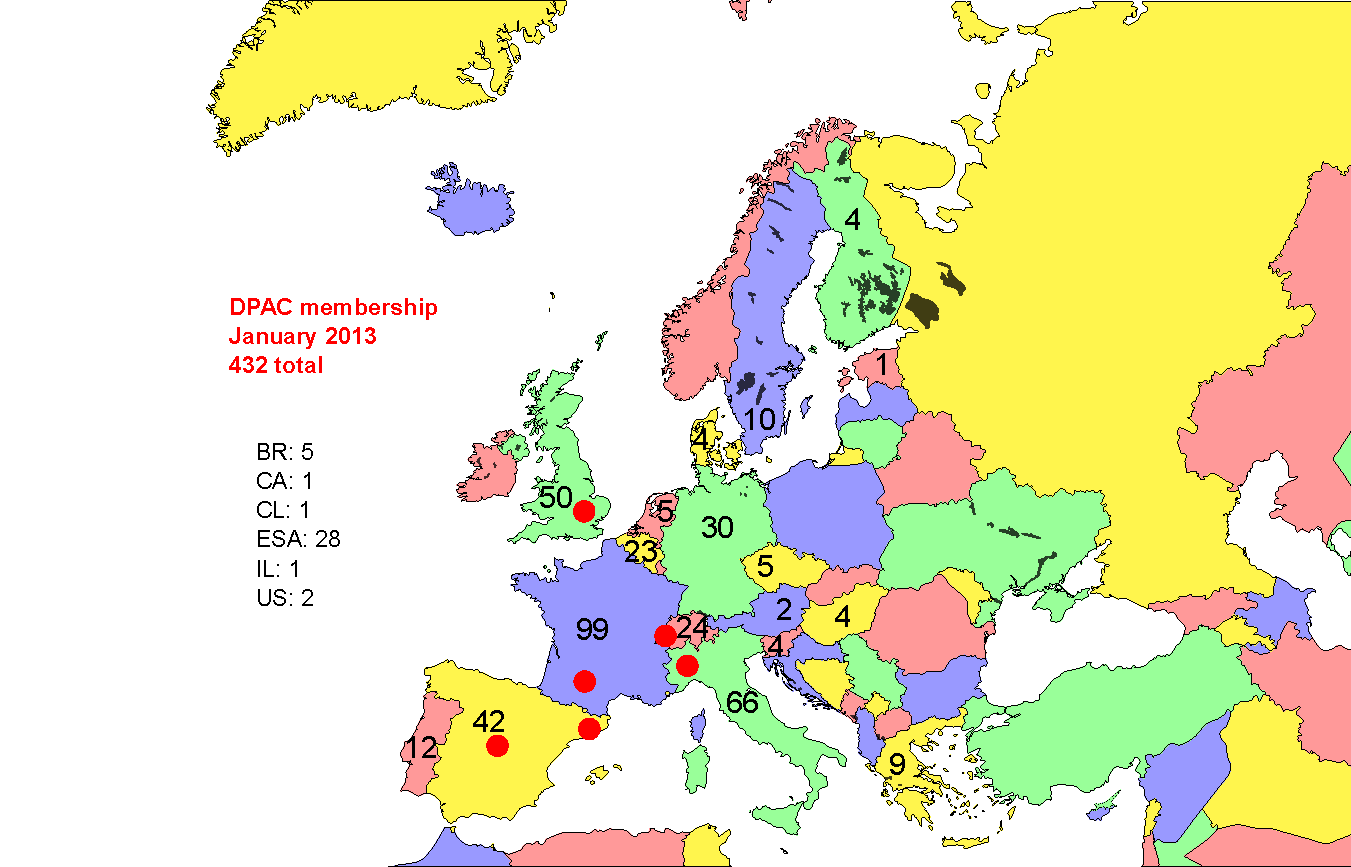
\includegraphics[height=\paperheight]{images/DpacMembershipMapAndDPCs.pdf}};
    \node at ($(map.north west)+(4,-1.7)$)
    {
\includegraphics[height=1.3cm]{images/dpac_logo.pdf}};
    \node at ($(map.north east)-(0.1,0.5)$) [anchor=north east, text width=4.8cm, text badly ragged,
    fill=white, fill opacity=0.8, text opacity=1, rounded corners=5pt]
    {\begin{itemize}
      \item Gaia data processing is a Pan-European cooperation
        \begin{itemize}
          \item Over 1000 staff years effort since 2006
          \item Processing power spread over 6 centres
          \item Supported through national funding
          \item Additional support from EC Marie Curie and ESF
        \end{itemize}
    \end{itemize}
  };
  \node at ($(map.south east)+(-0.3,0.3)$) [anchor=south
  east]{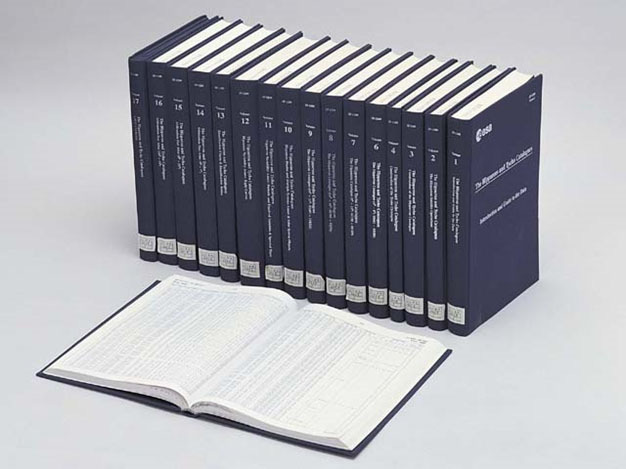
\includegraphics[height=3cm]{images/catalogue_hipparcos.pdf}};
\end{tikzpicture}
\end{emptyframe}


\frame {\frametitle{  In the beginning} 
\begin{itemize}
  \item initial ideas for ground segment were in place for the study in 2000 \citell{LL:ESA-SCI(2000)4}
  \item already clear then we would have distributed processing in multiple centres (though not mentioned)
  \item Intention was to have autonomy between coordination units
\pause
  \item Interviewed several project leaders for \cite{LL:WOM-003} in 2004/5 --- tried to learn from
    them \ldots
    \begin{itemize}
      \item Included LSST (Kantor) , SDSS (Borowski)
  \item Management came out as the most difficult part of all projects \ldots so I will leave that until last.
    \end{itemize}
  \item some things started before DPAC --- simulations and GIS studies for example.
  \item Finally DPAC is large --- I am sure you can find someone in DPAC to disagree with anything I say. 
\end{itemize}
}


\section{Standards and Tools}

\frame {\frametitle{  Language (spoken) and conventions } 
\begin{itemize}
  \item Very important in large groups
  \item Which way is up on Gaia, which is a row and column on focal plane, which quaternion to use
  \item {\color{green} dealt with quite early on in \citell{LL:BAS-003}}
    \begin{itemize}
      \item still Astrium have a different definition for $X,Y,Z$ on Gaia
      \item at least in the consortium there is only one  --- could have been much worse  
    \end{itemize}
    \pause
  \item What is a product, a Work Package --- why is 10 months $=$ 1 year
  \item also dealt with early on in \citell{LL:WOM-001}
    \pause
  \item Then there are Acronyms \url{http://gaia.esac.esa.int/gpdb/glossary.txt} and an acronym tool
    for TeX files (e.g. Appendix \ref{sect:acr})
    \pause
  \item having a complete engineering guideline early was good \citell{LL:JH-001}
\end{itemize}
}


\frame {\frametitle{ Parameters and data models } 
\begin{itemize}
%\item Which value do we use for speed of light, measurements of Gaia instrument 
  \item Avoid different values of constants in peoples code \ldots 
  \item The Gaia Parameter Database was set up early on for this \citep{2005ESASP.576...67D}
    \begin{itemize}
      \item all constants in one place; web searchable configuration controlled (Only updated by Jos De Bruijne)
      \item published as constants for Java (can also do C, Fortran\ldots) so you may refer to a particular version
    \end{itemize}
  \item then the actual data model --- what exactly is an AstroElementary?
    \begin{itemize}
      \item entire data model defined in multi-user dictionary tool; includes Units on each field.
        \begin{itemize}
          \item good for astronomers --- computer people find it harder to handle 
        \end{itemize}
      \item from it we generate data instance classes and schemas for storage.
      \item {\color{green} ONLY data model not processing} --- all objects are dumb (had discussion with KT  and Mario on this)
%	\item This was in UML (Rose) in the 90s but it was impractical to continue..
    \end{itemize}
  \item {\color{green} These are logical extensions of having agreed conventions\ldots}
\end{itemize}
}

\frame {
  \frametitle{  Flight Operations Procedures in MOC}
\vspace{-0.5cm}
\begin{center}	
   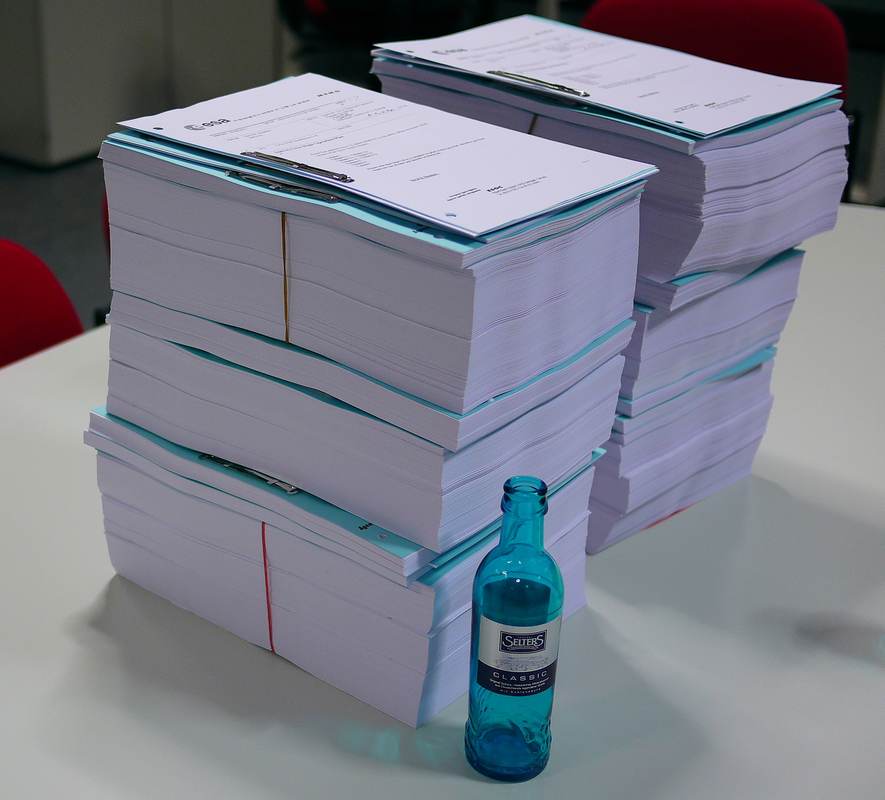
\includegraphics[width=0.6\textwidth,trim=0cm 0cm 0cm 0cm]{images/fops}\\
\end{center}
\vspace{-15pt}
The FOP is followed by the spacecraft operators - the paper copy is just in case the computers fail - could be useful! 
{\color{red} But we should avoid {\em write only} documents.}
}

\frame {\frametitle{ Have a standard: DPAC follows ECSS }
\begin{columns}
  \begin{column}{0.5\textwidth}
%\pgfputat{\pgfxy(0,0)}{\pgfbox[left,top]{
    %\begin{center}
      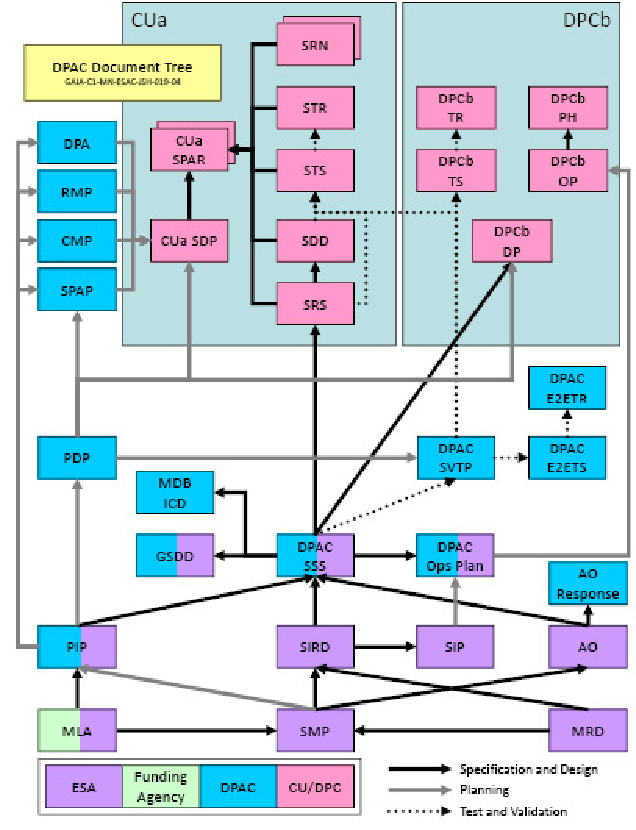
\includegraphics[width=0.9\textwidth]{images/doctree-crop}\\
    %\end{center}
      {\tiny Doctree by  John Hoar \citellp{LL:RD-010}}\hfill
%}}
  \end{column}
  \begin{column}{0.5\textwidth}
    \vskip-7.3cm
    \textbf{European Cooperation for Space Standardization}
    \begin{itemize}
      \item ECSS tailored as in figure
        \begin{itemize}
          \item LaTeX Templates/examples provided (by SOC) 
          \item Documents are iterated ---  All of this is done for all DPAC products.
          \item {\color{green} It is very good to have a standard set of documents augmented by technical notes and streamlined ECSS}
          \item Some still found it too heavy --- other reports requested beyond the standard ones.
        \end{itemize}
      \item DPAC had sufficient QA people ($\sim1/$CU) from the start to help with this% and create examples and templates.
    \end{itemize}
  \end{column}
\end{columns}
}

\frame {\frametitle{  LSST  DM docs } 

\begin{itemize}
  \item  No standard - no Overview  of DM docs I could find  some web pages 
\begin{itemize}
  \item LDM-493 .. covers some aspects .. but still no Doctree - templates ?
  \item not nice to have tex/markdown/word others ?   Markdown ok for implementation docs but for technotes for science notes?  
   \item did not find a document management plan for DM .. 
\end{itemize}
  \item Mention made of LPM-051 .. but is DM following this ? Or just not declaring controlled documents .. prefer term ISSUED rather than controlled
	\begin{itemize}

   \item docushare  is the LSST repo but DM docs seem old (did find some from KT) - should all issued docs be there (I think so ..)
	\item would expect to find all Technotes from DM in docushare .. like in a technotes folder ... SQR-006 gives an API which I may be able to use - should not be this hard.
	\end{itemize}
\item would like to find all draft docs in one DM repo .. 
    \item everything is {\em referenceable} - but I do not find a single bibtex database or such for issued docs ..  (Gaia livelink metadata is exported as a bibtex every night) 
\end{itemize}
}
\frame {\frametitle{  LSST  DM docs } 
\begin{itemize}
  \item  LDTN-030 - ok for code documentation -  understand its evolving- 
	\begin{itemize}
	\item overlaps LDM-493 somewhat - Why so many documentation projects - should we have ONE for DM ?
	\item Provides document shards - no structure - how do you get a an old version (users will not get from git) .. LTD perhaps - but not well explained.
	\item All products should be listed and for each product the set of docs .. the Audience seems too broad to cover with one type of document.
	
	\item This "In our case, the situation is complicated by the fact that Data Management software is being built by multiple teams across many coupled repositories. Taken together, the software repositories of the Data Management System are typically called the Stack, but not all parts of the Stack are used together. There are server-side database and display components, as well as pipelines algorithms bound together with middle ware." {\color{red} does not sound like good system engineering is in place .. }
	\item Unclear in a massive web how one  can check consistency to any given level for docs .. {\color{red} Potential  problem for reviewers}
	\end{itemize}
\end{itemize}
  
}



\frame {\frametitle{ Single Sign on  Gaia Portal } 
\begin{itemize}
  \item \url{http://www.rssd.esa.int/index.php?project=MYPORTAL&page=index} hosted at ESTEC; set up
    eons ago\ldots
  \item Names, emails and affiliations (phone numbers, photo, address) of all Gaia people
  \item Single login (LDAP) for 
    \begin{itemize}
      \item Livelink --- for all published documents
      \item Wiki --- for wiki things (meeting setup etc.); always draft nearly always out of date
      \item Mantis --- for all issues 
    \end{itemize}
  \item Same LDAP for SVN, MDB dictionary etc
  \item Single sign on is perhaps not great but having one LDAP for authentication of everything
    is fabulous!
  \item {\color{blue} Having information in SVN, Livelink and possibly on a wiki is not great but we
  do not have a solution}
  \item {\color{green} Having single agreed set of collaboration tools from the outset excellent.}
\end{itemize}
}

\frame{\frametitle{Development tools}
\begin{itemize}
  \item All DPAC code and docs in Subversion, hosted at ESAC 
    \begin{itemize}
      \item Access control according to Group membership in the LDAP 
    \end{itemize}
  \item Mantis for centralised issue tracking (includes risks and actions)
    \begin{itemize}
      \item ALL DPAC issues in one system hosted at ESTEC 
      \item {\color{red} Jira would probably be better }
  \end{itemize}
\pause
  \item{\color{green} Having one language is good \citep{2011arXiv1108.0355O}} agreed 2006

    \citellp{LL:JH-001} --- only one verification part is NOT in Java. 
    \begin{itemize}
      \item Can have a library of standard  routines  GaiaTools (Relativity, Field Angle Calculator,
        Ephemeris handling\ldots)
        \begin{itemize}
          \item {\color{red} The set of routines were not defined hence GaiaTools is a bit of
          hodgepodge mess\ldots}
          \item {\color{blue} Counter argument for common tools is (unnecessary)
          interdependence\ldots}
        \end{itemize}
      \item all libs in Nexus 
      \item builds with Ant; {\color{red} Maven might be the thing to use now}
      \item automated builds with Hudson/Jenkins (previously cruisecontrol)
      \item {\color{blue} virtual machines make some reasons for Java invalid}
    \end{itemize}
\end{itemize}
}



